\chapter{Opdracht}

\textit{In dit hoofdstuk wordt de opdracht uitgelegd zoals gegeven door Quintor. Het betreft de aanleiding van de opdracht en het uiteindelijke doel Quintor wilt behalen door het faciliteren van de afstudeeropdracht.}

Sinds de opkomst van Bitcoin is de Blockchain technologie, de techniek die het mogelijk maakt om het op een gedecentraliseerde manier te laten werken, steeds populairder geworden. Alhoewel de Blockchain-technologie nog in de kinderschoenen staat, gaan de ontwikkelingen in het domein zeer snel. Zo worden er toepassingen bedacht die niet alleen voor de financiële markten interessant zijn, maar ook voor bijvoorbeeld het digitaliseren van contracten en contractbeheer. 

Door de snelle groei van het Blockchain domein heeft Quintor in 2017 in samenwerking met DUO/MinOCW, Groningen Declaration Network, Stichting ePortfolio Support, TNO en Rabobank, het Blockchain Field-lab Education gestart in Groningen. Het Blockchain-lab is opgezet om expertise en kennis uit te wisselen op regionaal, nationaal en internationaal gebied. De oprichting van het Blockchain Field-lab Education heeft er mede voor gezorgd dat Quintor afstudeeropdrachten aanbiedt voor het Blockchain domein om zo de huidige kennis over het domein uit te breiden en/of te toetsen.

\begin{figure}[h]
  \centering
  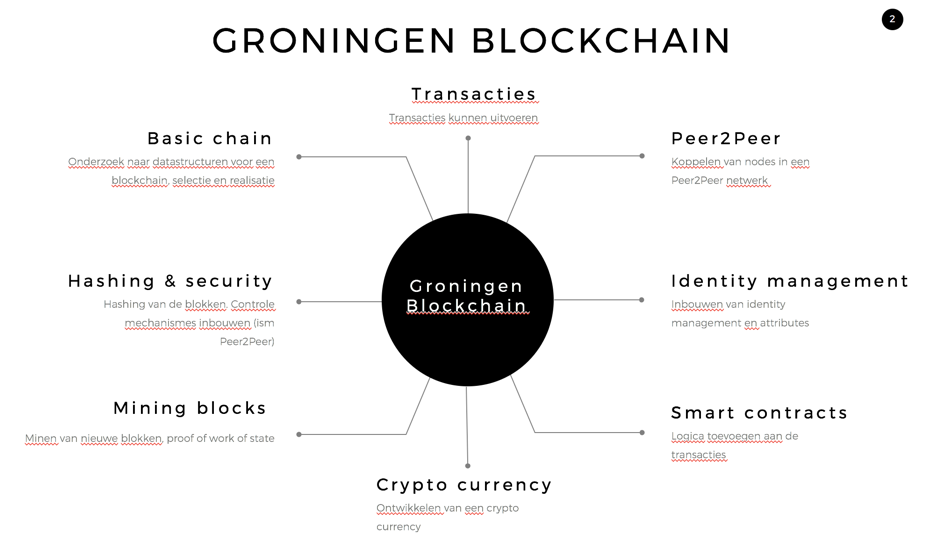
\includegraphics{figures/indeling_blockchain_opdracht}
  \caption[Indeling opdracht Blockchain Quintor.]{
    De indeling van de Blockchain opdracht zoals gegeven door Quintor. Door het domein op te delen in segmenten is het mogelijk om elk individueel segment uit te lichten in de vorm van onderzoek, zoals te zien in bijlage \ref{appendix:opdrachtformulering}.
  }
  \label{fig:indeling_blockchain_opdracht} 
\end{figure}

\clearpage
Aangezien het Blockchain domein complex en veelomvattend is, is het domein opgedeeld in segmenten. De verschillende segmenten, zoals weergegeven in fig. \ref{fig:indeling_blockchain_opdracht}, worden aangeboden als individuele afstudeeropdrachten. De focus van deze opdracht zijn de segmenten Peer2Peer en Identity Management, waarbij door middel van gestelde uitgangspunten op het gebied van snelheid, beveiligingsniveau en toepassingsmogelijkheden een Proof of Concept gerealiseerd dient te worden. Alvorens het Proof of Concept gerealiseerd kan worden, worden de alternatieve architecturen op het gebied van Peer2Peer en Identity Management in kaart gebracht. Dit wordt gedaan door het uitvoeren van literatuur onderzoek naar keuzes die gemaakt zijn in huidige Blockchain implementaties.

Daarnaast worden de volgende eisen gesteld aan het Proof of Concept:
\begin{enumerate}[noitemsep]
  \item Er worden geen Blockchain libraries gebruikt.
  \item Het moet resistent zijn tegen aanvallen.
  \item Het moet gedistribueerd zijn.
  \item Er wordt op decentrale wijze consensus bereikt.
\end{enumerate}

\section{Probleemstelling}

Doordat de toepassing en adoptie van Blockchain technologie steeds groter wordt wil Quintor de toepassingsmogelijkheden en technieken onderzoeken om te kijken of het haalbaar is om een Blockchain implementatie te realiseren, waarna er gekeken zal worden of Quintor de technologie kan gebruiken in vraagstukken vanuit klanten.

\section{Doelstelling}

Door het Blockchain domein op te delen in segmenten, te zien in fig. \ref{fig:indeling_blockchain_opdracht}, is het mogelijk om de segmenten te behandelen in afstudeeropdrachten die Quintor aanbiedt. De focus in deze opdracht ligt op de Blockchain onderdelen Identity Management en Peer2Peer (Distributed Network). Hierdoor is er een globaal doel en een doel die specifiek voor deze opdracht geldt. Het streven van het globale doel is het opdoen van kennis omtrent het realiseren van een Blockchain implementatie door het creëren van individuele segmenten. Het doel van deze specifieke opdracht is middels het opstellen van een Proof of Concept van de Blockchain onderdelen Identity Management en Distributed Network, zonder gebruik te maken van bestaande Blockchain oplossingen, kennis te ontwikkelen voor Quintor op het gebied van Blockchain technologie.

\section{Resultaat}

Indien de opdracht succesvol afgerond is, zijn de segmenten Identity Management en het Distributed Network gerealiseerd in de vorm van een Proof of Concept en voldoen aan de eisen die gesteld zijn in de opdrachtformulering. Dit Proof of Concept zal werken met de segmenten, Basic Chain, Hashing \& security en Mining blocks, die gerealiseerd zullen worden door Kevin Bos. Zowel het Proof of Concept als het onderzoek zal voor Quintor inzicht bieden in het Blockchain domein en de ontwikkelingen daarin.

\subsection{Producten}

Als onderdeel van de afstudeeropdracht zullen er verschillende producten worden opgeleverd aan Quintor en aan de Haagse Hogeschool. Deze staan hieronder gespecificeerd.

De op te leveren producten aan Quintor zijn:
\begin{itemize}
  \item{\textbf{Adviesrapport}}
  \\ Presentatie over de resultaten van het onderzoek waarin verschillende technieken geadviseerd worden die toegepast zijn in de realisatie van het Proof of Concept.
  \item{\textbf{Sprint demo presentaties}}
  \\ Elke twee weken zal er een presentatie gegeven worden over de voortgang van het project waarbij het mogelijk is om feedback te krijgen over blokkades of aanpakken.
  \item{\textbf{Broncode van het Proof of Concept}}
  \\ De gehele broncode van de applicatie waarin technieken vanuit het adviesrapport gerealiseerd zijn.
  \item{\textbf{Onderzoeksrapport}}
  \\ De resultaten van het onderzoek dat uitgevoerd is om inzicht te krijgen in de segmenten Distributed Network en Identity Management.
\end{itemize}

\newpage
De op te leveren producten aan de Haagse Hogeschool zijn:
\begin{itemize}
  \item{\textbf{Afstudeerscriptie}}
  \\ Beschrijving van het proces tijdens de uitvoering van de afstudeeropdracht ter beoordeling van de bekwaamheid van de student en de geselecteerde beroepstaken.
  \item{\textbf{Verslag bedrijfsbezoek}}
  \\ Verslag van het bedrijfsbezoek dat tijdens het afstudeertraject gedaan wordt.
  \item{\textbf{Voortgangsverslag}}
  \\ Verslag van de voortgang van de afstudeeropdracht.
\end{itemize}


